\usetikzlibrary{arrows.meta,shapes.multipart,patterns,positioning}
\begin{frame}[fragile,label=vm]{recall(?): virtual memory}
\begin{itemize}
\item illuision of \myemph{dedicated memory}
\end{itemize}
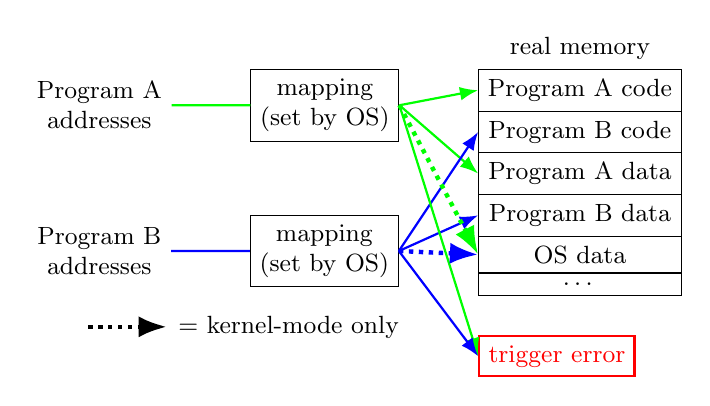
\begin{tikzpicture}
\tikzset{
    every node/.style={font=\small},
}
\node[align=center] (progAAddr) {Program A \\ addresses};
\node[below=1cm of progAAddr,align=center] (progBAddr) {Program B \\ addresses};
\node[draw, right=1cm of progAAddr,align=center] (translationA) { mapping \\ (set by OS) };
\node[draw, right=1cm of progBAddr,align=center] (translationB) { mapping \\ (set by OS) };
\node[draw,rectangle split, rectangle split parts=6, anchor=north west,label={north:real memory}] (mem) at ([xshift=1cm]translationA.north east) {
    \nodepart{one}
    Program A code 
    \nodepart{two}
    Program B code
    \nodepart{three}
    Program A data
    \nodepart{four}
    Program B data
    \nodepart{five}
    OS data
    \nodepart{six}
    \ldots
};
\draw[-Latex,green,thick] (progAAddr) -- (translationA) (translationA.east) -- (mem.one west);
\draw[-Latex,green,thick] (translationA.east) -- (mem.three west);
\draw[-Latex,blue,thick] (progBAddr) -- (translationB) (translationB.east) -- (mem.two west);
\draw[-Latex,blue,thick] (translationB.east) -- (mem.four west);
\node[thick,red,draw,anchor=north west] (error) at ([yshift=-.5cm]mem.south west) {trigger error};
\draw[-Latex,green,thick] (translationA.east) -- (error.west);
\draw[-Latex,blue,thick] (translationB.east) -- (error.west);
\draw[-Latex,green,ultra thick,dotted] (translationA.east) -- (mem.five west);
\draw[-Latex,blue,ultra thick,dotted] (translationB.east) -- (mem.five west);
\draw[-Latex,ultra thick,dotted] ([xshift=-3cm,yshift=-.5cm]translationB.south) -- ([xshift=-2cm,yshift=-.5cm]translationB.south)
    node[right] {= kernel-mode only};
\end{tikzpicture}
\end{frame}

